\section{长期分布与时间平均}
\label{sec:dtsp-long-run}

现在回到第~\ref{sec:dtsp-visits}节留下的问题：链运行很久以后会怎样。这里有两个不同的问题。其一，某个很晚的时刻$n$，状态$X_n$服从什么分布，它是否趋向不变分布，速度多快？其二，沿一条长轨迹计算平均$\frac1n\sum_{k<n}f(X_k)$，它是否趋向某个常数，误差有多大？前者关心的是“很多次独立重复运行、在同一时刻拍快照”，后者关心的是“一次运行、沿时间累计”。周期链已经表明二者可以不同：快照分布永远振荡，时间平均却收敛。本节先用时间平移描述“统计规律不变”，再分别研究这两个问题。

\subsection{平稳性与时间平移}
\label{sec:dtsp-stationarity}

\paragraph{严格平稳}
不变分布描述的是单个时刻的分布不变。更强的要求是：把整个观察窗口向后平移，所有时刻的联合规律都不变。

\begin{definition}[平稳过程]
  \label{def:dtsp-stationary-process}
  过程$(X_n)_{n\geq0}$称为（严格）\term{平稳过程}（stationary process），若对任意正整数$m$、时刻$n_1,\ldots,n_m\geq0$和平移量$h\geq0$，
  \[
    (X_{n_1},\ldots,X_{n_m})\overset{\mathrm d}{=}(X_{n_1+h},\ldots,X_{n_m+h}).
  \]
\end{definition}

\begin{theorem}[从不变分布启动的链是平稳的]
  \label{thm:dtsp-stationary-chain}
  设$(X_n)$是以$P$为转移核的时间齐次Markov链，$X_0\sim\pi$且$\pi P=\pi$。则$(X_n)$是平稳过程。
\end{theorem}

\begin{proof}
只需检查连续窗口$(X_h,\ldots,X_{h+m})$的规律不依赖$h$，因为任意有限组时刻都是某个连续窗口的边缘。由Markov性质，这一窗口的联合规律是$\mu_h(\mathrm dx_0)P(x_0,\mathrm dx_1)\cdots P(x_{m-1},\mathrm dx_m)$，其中$\mu_h$是$X_h$的分布。而$\mu_h=\pi P^h=\pi$，所以联合规律与$h$无关。
\end{proof}

只知道某一时刻的边缘等于$\pi$并不够：上面的论证同时用到了核不变与Markov结构。例如图~\ref{fig:dtsp-ar1-path-bundle}中的递推若从$X_0\sim\mathcal N(0,1/0.36)$启动，每个$X_n$都服从同一个正态分布，而且整个过程平稳；两步之间的协方差为$\operatorname{Cov}(X_n,X_{n+k})=0.8^k/0.36$，只依赖间隔$k$。平稳并不意味着独立，相邻读数仍以$0.8$的系数相关。

\paragraph{二阶平稳}
若只计算均值和二阶误差，可以只要求均值不变、协方差只依赖时间差。具有有限二阶矩的实值过程若$\mathbb EX_n$与$n$无关、$\operatorname{Cov}(X_n,X_{n+k})$只依赖$k$，称为\term{二阶平稳}（second-order stationarity），也称弱平稳。严格平稳且二阶矩有限蕴含二阶平稳；反之不成立。取相互独立的序列，偶数时刻服从标准正态，奇数时刻等概率取$\pm1$：均值都是零，方差都是一，不同时刻的协方差都是零，所以二阶平稳；但一维边缘随奇偶改变，不是严格平稳。联合高斯过程的有限维分布由均值与协方差完全确定，对它们二者等价。二阶平稳过程的频谱表示与线性滤波属于信号与状态估计部分，这里不展开。

\paragraph{平稳过程与平稳增量}
公平游走$S_n$的方差为$n$，随时间增长，不是平稳过程；但它的增量$\xi_n$独立同分布，因而增量过程平稳。类似的区分对连续时间的Brownian运动同样重要。同一个公平游走因此同时是Markov链、鞅，且具有平稳增量，而它本身不平稳：这几种结构回答不同的问题，并不互斥。

\subsection{Markov链的分布收敛}
\label{sec:dtsp-distribution-convergence}

\paragraph{用总变差比较分布}
要说$X_n$的分布“接近”$\pi$，先要有一个比较分布的尺度。最直接的尺度是：有没有某个事件，两个分布给它的概率差得很多。对同一可测空间上的概率测度$\mu,\nu$，定义
\[
  \lVert\mu-\nu\rVert_{\mathrm{TV}}=\sup_{B\in\mathcal E}|\mu(B)-\nu(B)|,
\]
称为\term{总变差距离}（total variation distance）。可数状态时它等于$\frac12\sum_i|\mu_i-\nu_i|$：令$B^\ast=\{i:\mu_i>\nu_i\}$，两者总质量相等，故$\mu(B^\ast)-\nu(B^\ast)=\frac12\sum_i|\mu_i-\nu_i|$；对任意$B$，$\mu(B)-\nu(B)\leq\mu(B\cap B^\ast)-\nu(B\cap B^\ast)\leq\mu(B^\ast)-\nu(B^\ast)$，另一侧对称。总变差为$0.01$意味着没有任何事件的概率被改变超过$0.01$。概率分布之间更一般的距离与几何留到概率分布部分，本章只用这一种。

\paragraph{耦合：让两条链相遇}
怎样证明从$x$出发的链“忘记”了起点？一个形象的办法是让两个人同时在转移图上随机行走，一个从$x$出发，另一个从$\pi$中随机选起点。两人各自独立行走，一旦站在同一个状态，就从此手拉手一起走。相遇以后两人的位置永远相同；而第二个人始终服从$\pi$，因为$\pi$不变。于是第一个人在时刻$n$的分布与$\pi$的差别，不会超过“到时刻$n$两人还没相遇”的概率。

把这一想法写成不等式。若随机对$(X,Y)$满足$X\sim\mu$、$Y\sim\nu$，则对任意$B$，$\mu(B)-\nu(B)=\mathbb P(X\in B)-\mathbb P(Y\in B)\leq\mathbb P(X\in B,Y\notin B)\leq\mathbb P(X\neq Y)$，因此
\begin{equation}
  \lVert\mu-\nu\rVert_{\mathrm{TV}}\leq\mathbb P(X\neq Y).
  \label{eq:dtsp-coupling-inequality}
\end{equation}
上面的“手拉手”构造中，第二条链在相遇时刻（一个停时）之后改为跟随第一条链，由强Markov性质它仍是以$P$为转移核的链。若$T$是相遇时刻，便有$\lVert P^n(x,\cdot)-\pi\rVert_{\mathrm{TV}}\leq\mathbb P(T>n)$。剩下的问题是让相遇足够快，下面用一步一步的“最大重合”把它量化。

\paragraph{一步转移的收缩系数}
对转移核$Q$，定义\term{Dobrushin系数}（Dobrushin coefficient）
\[
  \delta(Q)=\sup_{x,x'}\lVert Q(x,\cdot)-Q(x',\cdot)\rVert_{\mathrm{TV}}.
\]
它度量“从两个最不相同的起点出发，走一步后的分布最多还差多少”。可数状态时，$\delta(Q)=1-\min_{x,x'}\sum_y\min\{Q(x,y),Q(x',y)\}$：每对行向量的公共部分越多，一步后越难分辨起点。

\begin{lemma}[总变差的收缩]
  \label{lem:dtsp-dobrushin}
  对可数状态上的概率分布$\mu,\nu$与转移核$Q$，$\lVert\mu Q-\nu Q\rVert_{\mathrm{TV}}\leq\delta(Q)\lVert\mu-\nu\rVert_{\mathrm{TV}}$。
\end{lemma}

\begin{proof}
记$t=\lVert\mu-\nu\rVert_{\mathrm{TV}}$，设$t>0$。差$\mu-\nu$的正部与负部总质量都是$t$，于是可写$\mu-\nu=t(\alpha-\beta)$，其中$\alpha,\beta$是概率分布。从而
\[
  \mu Q-\nu Q=t(\alpha Q-\beta Q)=t\sum_{x,x'}\alpha_x\beta_{x'}\bigl(Q(x,\cdot)-Q(x',\cdot)\bigr).
\]
可数状态上$\lVert\cdot\rVert_{\mathrm{TV}}$等于半个$\ell^1$范数，满足三角不等式，故右侧的总变差至多$t\sum_{x,x'}\alpha_x\beta_{x'}\delta(Q)=t\,\delta(Q)$。
\end{proof}

对两状态链~\eqref{eq:dtsp-two-state-matrix}，两行的公共部分为$\min(0.9,0.2)+\min(0.1,0.8)=0.3$，所以$\delta(\bm P)=0.7$，恰好是式~\eqref{eq:dtsp-two-state-power}中的衰减率。确定交替链的两行没有公共部分，$\delta=1$，而且对所有$n$都有$\delta(\bm P^n)=1$：它永远不收缩。周期正是使所有幂的行向量支撑错开的结构。

\paragraph{有限非周期链的几何收敛}
要让某个幂$\bm P^m$的任意两行都有公共部分，只需$\bm P^m$的每个元素都为正。非周期性恰好保证这一点。

\begin{lemma}[非周期链的正幂]
  \label{lem:dtsp-positive-power}
  有限、不可约、非周期的转移矩阵$\bm P$存在整数$m$，使$\bm P^m$的所有元素严格为正。
\end{lemma}

\begin{proof}
固定状态$i$，返回步数集$R_i$对加法封闭（先走一个回路再走另一个），且$\gcd R_i=1$。先证$R_i$包含所有足够大的整数。取有限个元素使其最大公约数为$1$，由Bezout等式存在整数系数把$1$写成它们的组合；把正系数项与负系数项分开，得到$A,B\in R_i\cup\{0\}$使$A-B=1$。若$B=0$则$1\in R_i$，结论平凡。否则对$n\geq B^2$，写$n=qB+r$，$0\leq r<B\leq q$，则$n=(q-r)B+rA\in R_i$。于是存在$N_i$使$n\geq N_i$时$P^n(i,i)>0$。对任意$j$取$k_{i,j}$使$P^{k_{i,j}}(i,j)>0$，则$n\geq N_i+k_{i,j}$时$P^n(i,j)\geq P^{n-k_{i,j}}(i,i)P^{k_{i,j}}(i,j)>0$。取$m=\max_{i,j}(N_i+k_{i,j})$即可。
\end{proof}

\begin{theorem}[有限链的几何遍历]
  \label{thm:dtsp-finite-convergence}
  设有限状态转移矩阵$\bm P$不可约、非周期，$\pi$为其不变分布，$m$如引理~\ref{lem:dtsp-positive-power}，并令
  \[
    \beta=\min_{x,x'}\sum_y\min\{P^m(x,y),P^m(x',y)\}>0 .
  \]
  则对任意初始分布$\mu$和所有$n\geq0$，
  \begin{equation}
    \lVert\mu P^n-\pi\rVert_{\mathrm{TV}}\leq(1-\beta)^{\lfloor n/m\rfloor}.
    \label{eq:dtsp-geometric-ergodicity}
  \end{equation}
\end{theorem}

\begin{proof}
由$\pi=\pi P^n$，$\lVert\mu P^n-\pi\rVert=\lVert\mu P^n-\pi P^n\rVert$。写$n=qm+r$，反复使用引理~\ref{lem:dtsp-dobrushin}，其中$\delta(\bm P^m)=1-\beta$，$\delta(\bm P^r)\leq1$，并用$\lVert\mu-\pi\rVert\leq1$。
\end{proof}

这个定理顺便再次证明了不变分布唯一：两个不变分布之间的距离也被压缩，只能为零。最坏初态下的距离$d(n)=\sup_x\lVert P^n(x,\cdot)-\pi\rVert_{\mathrm{TV}}$关于$n$单调不增，对$0<\varepsilon<1$，称$t_{\mathrm{mix}}(\varepsilon)=\min\{n:d(n)\leq\varepsilon\}$为\term{混合时间}（mixing time）。具有几何衰减界$\lVert P^n(x,\cdot)-\pi\rVert_{\mathrm{TV}}\leq C(x)r^n$（$r<1$）的链称为满足\term{几何遍历性}（geometric ergodicity）。

图~\ref{fig:dtsp-tv-decay}在对数纵轴上画出几条链的$d(n)$。两状态链精确地有$d(n)=\frac23\times0.7^n$，是一条直线。在$m$个点组成的环上，每步以$1/2$停留、各以$1/4$向两侧移动（称为惰性环），$d(n)$同样几何下降，但斜率小得多：$m=12$时$d(50)\approx0.019$，$m=24$时$d(50)\approx0.27$。环长加倍，混合所需步数大约变成四倍，这是“扩散”的典型尺度：随机游走走过距离$m$需要约$m^2$步。去掉停留概率的非惰性环在$m$为偶数时周期为$2$，$d(n)$停在$1/2$不动。

\begin{figure}[htbp]
  \centering
  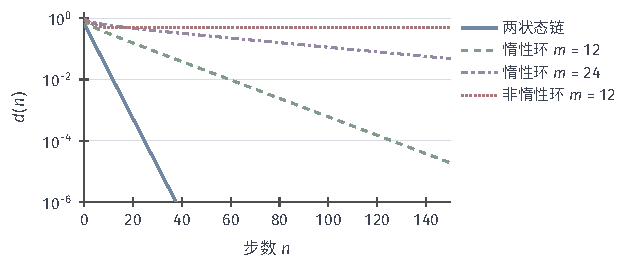
\includegraphics[width=106mm]{figures/03-optimization-evolution-and-signals/02-processes-and-trajectory-evolution/tikz/dtsp-tv-decay/figure.pdf}
  \caption{最坏初态到平稳分布的总变差$d(n)$（精确计算，纵轴对数刻度）。两状态链为$\frac23\times0.7^n$；惰性环每步以$1/2$停留、各以$1/4$移向两个邻点，$m$为环上状态数；非惰性环各以$1/2$移向两个邻点，$m=12$时周期为$2$，$d(n)$恒为$1/2$。}
  \label{fig:dtsp-tv-decay}
\end{figure}

\paragraph{谱的视角}
Dobrushin系数给出的速度常常保守。对可逆链，转移矩阵的谱给出更精细的刻画。在加权内积$\langle f,g\rangle_\pi=\sum_i\pi_if(i)g(i)$下，细致平衡等价于$\langle Pf,g\rangle_\pi=\langle f,Pg\rangle_\pi$，即$P$是自伴算子，因此特征值都是实数，可排为$1=\lambda_1\geq\lambda_2\geq\cdots\geq\lambda_{|E|}\geq-1$。

\begin{theorem}[可逆链的谱界]
  \label{thm:dtsp-spectral-bound}
  设有限链不可约且关于$\pi$可逆，$\lambda_\ast=\max\{|\lambda|:\lambda\text{为特征值},\lambda\neq1\}$。则对每个状态$x$，
  \[
    \lVert P^n(x,\cdot)-\pi\rVert_{\mathrm{TV}}\leq\frac12\sqrt{\frac{1-\pi_x}{\pi_x}}\,\lambda_\ast^n.
  \]
\end{theorem}

\begin{proof}
令$h_n(y)=P^n(x,y)/\pi_y$。由细致平衡，$h_n=P^nh_0$，其中$h_0=\mathbb I_{\{x\}}/\pi_x$；并且$h_0-1$与常数函数在$\langle\cdot,\cdot\rangle_\pi$下正交。$P$限制在与常数正交的子空间上范数为$\lambda_\ast$，故$\lVert h_n-1\rVert_\pi=\lVert P^n(h_0-1)\rVert_\pi\leq\lambda_\ast^n\lVert h_0-1\rVert_\pi=\lambda_\ast^n\sqrt{(1-\pi_x)/\pi_x}$。最后由Cauchy--Schwarz，$2\lVert P^n(x,\cdot)-\pi\rVert_{\mathrm{TV}}=\sum_y\pi_y|h_n(y)-1|\leq\lVert h_n-1\rVert_\pi$。
\end{proof}

两状态链的另一个特征值是$0.7$；从状态$1$出发，界为$\frac12\sqrt{1/2}\times0.7^n\approx0.354\times0.7^n$，与精确值$0.333\times0.7^n$相差无几。惰性环的特征值为$\frac12(1+\cos(2\pi k/m))$，$\lambda_\ast=\frac12(1+\cos(2\pi/m))$，$m=12$与$m=24$时分别约为$0.933$与$0.983$；$1-\lambda_\ast$称为谱间隙，它约以$m^{-2}$缩小，与图~\ref{fig:dtsp-tv-decay}中的斜率比较一致。负特征值接近$-1$对应近似周期的振荡，加入停留概率可以把谱推到非负。

\paragraph{一般状态空间：漂移与小集}
状态连续时，没有“矩阵的某个幂全为正”可用，但上面的两个要素仍有对应物。一是\term{漂移条件}（drift condition）：存在函数$V\geq1$、常数$\lambda<1$、$b<\infty$与集合$C$，使
\[
  PV(x)\leq\lambda V(x)+b\,\mathbb I_C(x),
\]
即链在$C$外平均地被拉回来。二是$C$上的\term{小集}（small set）条件：存在$m\geq1$、$\beta>0$与概率测度$\nu$，使$P^m(x,\cdot)\geq\beta\nu(\cdot)$对所有$x\in C$成立，即从$C$中任一点出发，$m$步后的分布都包含一份共同的成分，耦合在每次回到$C$时都有至少$\beta$的机会成功。在这两项及适当的非周期条件下，链有唯一不变分布$\pi$，并且存在$r<1$与常数$K$，使$\lVert P^n(x,\cdot)-\pi\rVert_{\mathrm{TV}}\leq KV(x)r^n$\scite{math-meyn2009markov}。

用图~\ref{fig:dtsp-ar1-path-bundle}的递推核对这两项。取$V(x)=1+x^2$，则$PV(x)=1+\mathbb E(0.8x+\xi)^2=0.64V(x)+1.36$。在$C=\{|x|\leq2.6\}$之外$1.36\leq0.18V(x)$，所以$PV\leq0.82V+1.36\,\mathbb I_C$。在$C$上，$P(x,\cdot)$的密度$\varphi(y-0.8x)$不小于$\varphi(|y|+2.08)$，$\varphi$为标准正态密度，于是小集条件以$m=1$成立。因此这个递推几何遍历，与图中边缘分布迅速靠近$\mathcal N(0,1/0.36)$的观察一致。

\subsection{遍历平均与相关样本误差}
\label{sec:dtsp-ergodic-averages}
\label{sec:stoch-markov-long-run-average}

\paragraph{沿一条轨迹求平均}
模拟或监测通常只有一条长轨迹。我们希望用时间平均$\overline f_n=\frac1n\sum_{k=0}^{n-1}f(X_k)$近似$\pi(f)=\sum_i\pi_if(i)$，例如服务器长期处于拥堵状态的比例。困难在于各项彼此相关，不能直接套用独立同分布的大数定律。第~\ref{sec:dtsp-strong-markov}节的再生分段提供了出路：把轨迹在每次回到某个固定状态处切开，各段游程独立同分布，于是可以对“段”而不是对“步”使用大数定律。

\begin{theorem}[Markov链的遍历定理]
  \label{thm:dtsp-ergodic-theorem}
  设可数状态链不可约且正常返。则它有唯一的不变分布$\pi$，$\pi_i=1/m_i$；并且对任意初始分布和任意满足$\pi(|f|)<\infty$的$f$，
  \begin{equation}
    \frac1n\sum_{k=0}^{n-1}f(X_k)\longrightarrow\pi(f)\qquad\text{几乎必然}.
    \label{eq:dtsp-ergodic-average}
  \end{equation}
  特别地，有限不可约链（无论是否周期）都满足此结论。
\end{theorem}

\begin{proof}
固定状态$i$，先设$X_0=i$、$f\geq0$。记第$r$次返回$i$的时刻为$T^{(r)}$，$T^{(0)}=0$，常返性保证它们都有限。令$L_r=T^{(r)}-T^{(r-1)}$为第$r$段游程的长度，$F_r=\sum_{k=T^{(r-1)}}^{T^{(r)}-1}f(X_k)$为该段的累计值。由强Markov性质，$(L_r,F_r)_{r\geq1}$独立同分布，$\mathbb E_iL_1=m_i<\infty$。

第一步，识别段内平均。令$a_j=\mathbb E_i\sum_{k<T_i^{+}}\mathbb I\{X_k=j\}$为一段游程中访问$j$的平均次数，则$\sum_ja_j=m_i$，且由非负项换序，$\mathbb E_iF_1=\sum_ja_jf(j)$。向量$a$满足平衡方程：事件$\{k<T_i^+\}$属于$\mathcal F_k$，逐项对$\mathcal F_k$取条件期望，
\[
  \sum_\ell a_\ell P_{\ell,j}=\mathbb E_i\sum_{k=0}^{T_i^+-1}P_{X_k,j}=\mathbb E_i\sum_{k=0}^{T_i^+-1}\mathbb I\{X_{k+1}=j\}=\mathbb E_i\sum_{k=1}^{T_i^+}\mathbb I\{X_k=j\}=a_j,
\]
最后一步因为$X_0=X_{T_i^+}=i$，把计数区间平移一格不改变总数。所以$\tilde\pi=a/m_i$是不变分布，且$\mathbb E_iF_1=m_i\tilde\pi(f)$。

第二步，对游程使用强大数定律。若$\tilde\pi(f)<\infty$，则$\frac1R\sum_{r\leq R}F_r\to m_i\tilde\pi(f)$，$\frac1RT^{(R)}\to m_i$，几乎必然。记$R(n)$为时刻$n$之前完成的游程数，$T^{(R(n))}\leq n<T^{(R(n)+1)}$，且$R(n)\to\infty$。由$f\geq0$，
\[
  \frac{\sum_{r\leq R(n)}F_r}{T^{(R(n)+1)}}\leq\frac1n\sum_{k=0}^{n-1}f(X_k)\leq\frac{\sum_{r\leq R(n)+1}F_r}{T^{(R(n))}},
\]
两侧都趋于$\tilde\pi(f)$，因为$T^{(R+1)}/T^{(R)}\to1$。

第三步，推广。对一般初态$j$，链几乎必然在有限时间内到达$i$：否则从$i$出发以正概率到达$j$后永不返回，与$i$常返矛盾。到达前的有限段除以$n$后趋于零。对一般初始分布按$X_0$的取值分解，对$\tilde\pi$可积的一般$f$分成正负部分。

第四步，唯一性与$\pi_i=1/m_i$。若$\rho$是任一不变分布，令链从$\rho$出发；对有界$f$，$\mathbb E_\rho\overline f_n=\rho(f)$，而由已证结论$\overline f_n\to\tilde\pi(f)$几乎必然，有界收敛给出$\rho(f)=\tilde\pi(f)$。所以$\rho=\tilde\pi$，不变分布唯一，记作$\pi$。取$f=\mathbb I_{\{i\}}$，每段游程恰好访问$i$一次，$F_r=1$，得$\pi_i=1/m_i$。有限不可约链由第~\ref{sec:dtsp-communication}节为正常返，故适用。
\end{proof}

定理没有要求非周期，这正是图~\ref{fig:dtsp-two-state-distribution}(b)中交替链的时间平均趋于$1/2$的原因：时间平均只需要回返，逐时刻分布收敛还需要非周期。公式$\pi_i=1/m_i$说长期停留比例等于平均返回时间的倒数：两状态链中$m_1=3/2$、$m_2=3$，与$\pi=(2/3,1/3)$一致。一般状态空间中，正Harris常返链对任意初态和$\pi$可积的$f$有同样的结论\scite{math-meyn2009markov}；仅以正概率到达或只有局部可积，都不足以推出它。

\paragraph{平稳过程的遍历定理}
对一般的平稳过程（不必是Markov链），也有时间平均的极限定理：若$(X_n)$严格平稳且$\mathbb E|f(X_0)|<\infty$，则$\overline f_n$几乎必然收敛，但极限一般是随机的，等于$f(X_0)$对“平移不变事件”所成$\sigma$代数的条件期望；只有当所有平移不变事件的概率为$0$或$1$（称过程遍历）时，极限才是常数$\mathbb Ef(X_0)$\scite{math-kallenberg2021probability}。图~\ref{fig:dtsp-communicating-classes}的链提供了不遍历的例子：若初态随机地落在$\{3,4\}$或$\{5,6\}$中，由于两个类都封闭，长期平均取决于落在哪一个类，是一个随机极限。Markov链遍历定理中的不可约性正是排除这种情形的条件。

\paragraph{相关样本平均的方差}
遍历定理说明时间平均对准了$\pi(f)$；现在问有限$n$下误差有多大。设链从$\pi$启动，$\sigma_f^2=\operatorname{Var}_\pi f(X_0)\in(0,\infty)$，自相关$\rho_f(k)=\operatorname{Corr}_\pi(f(X_0),f(X_k))$。由平稳性，$\operatorname{Cov}(f(X_j),f(X_k))=\sigma_f^2\rho_f(|j-k|)$，展开平方并把相同间隔的项合并，
\begin{equation}
  \operatorname{Var}\bigl(\overline f_n\bigr)=\frac{\sigma_f^2}{n}\Bigl[1+2\sum_{k=1}^{n-1}\Bigl(1-\frac kn\Bigr)\rho_f(k)\Bigr].
  \label{eq:dtsp-average-variance}
\end{equation}
若$\sum_k|\rho_f(k)|<\infty$，方括号趋于$\tau_f=1+2\sum_{k\geq1}\rho_f(k)$，称为积分自相关时间。于是$n$个相关样本的平均，其方差约等于$n/\tau_f$个独立样本的平均，$n/\tau_f$称为\term{自相关有效样本量}（autocorrelation effective sample size）。它是针对特定$f$的方差换算口径，不是链中“真正独立”的样本条数；自相关为负时$\tau_f$还可能小于一。

对两状态链取$f=\mathbb I\{X=2\}$。$f-\pi(f)$在$\{1,2\}$上取$(-1/3,2/3)$，正比于特征向量$(1,-2)^{\top}$，所以$P(f-\pi f)=0.7(f-\pi f)$，从而$\rho_f(k)=0.7^k$，并且
\[
  \sigma_f^2=\frac13\cdot\frac23=\frac29,\qquad\tau_f=1+2\sum_{k\geq1}0.7^k=\frac{1.7}{0.3}=\frac{17}{3}.
\]
一条长$n$的轨迹提供的信息只相当于约$3n/17$个独立观测。图~\ref{fig:dtsp-ergodic-average}(a)中十条从状态$1$出发的轨迹的时间平均都收进$\frac13\pm2\sqrt{(2/9)(17/3)/n}$的带内，$n=4000$时带宽约为$\pm0.035$；(b)中长轨迹的经验自相关与$0.7^k$吻合。

\begin{figure}[htbp]
  \centering
  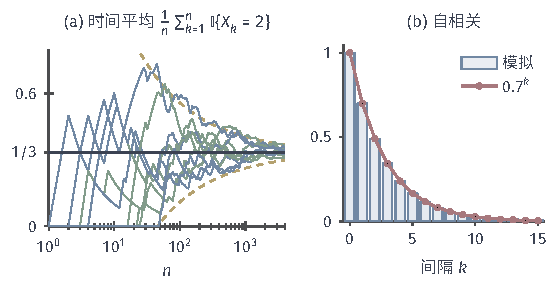
\includegraphics[width=94mm]{figures/03-optimization-evolution-and-signals/02-processes-and-trajectory-evolution/tikz/dtsp-ergodic-average/figure.pdf}
  \caption{两状态链的时间平均与自相关。(a)从状态$1$出发的$10$条模拟轨迹上，拥堵比例$\frac1n\sum_{k\leq n}\mathbb I\{X_k=2\}$随$n$的变化（横轴对数刻度）；黄色虚线为$\frac13\pm2\sqrt{\sigma_f^2\tau_f/n}$，$\sigma_f^2=2/9$、$\tau_f=17/3$。(b)一条长$200000$的模拟轨迹的经验自相关（柱）与精确值$0.7^k$（红线）。}
  \label{fig:dtsp-ergodic-average}
\end{figure}

\paragraph{Markov链的中心极限定理}
方差公式给出误差的尺度，误差的分布形状则需要中心极限定理。独立同分布情形的中心极限定理，以及用一致估计的标准误代替真值时的Slutsky定理，可参考\BookChapterRef{chap:weak-convergence-limit-theorems}{卷二“分布弱收敛、紧性与极限定理”章}。相关情形的关键一步，是把相关的和改写成鞅差的和。

对有限不可约链，方程
\begin{equation}
  g-Pg=f-\pi(f)
  \label{eq:dtsp-poisson-equation}
\end{equation}
有解$g$，称为链的\term{Poisson方程}（Poisson equation）。非周期时可以直接写出$g=\sum_{k\geq0}P^k(f-\pi f)$，定理~\ref{thm:dtsp-finite-convergence}保证级数几何收敛；周期情形也有解，只是需要另外构造。有了$g$，把$f(X_k)-\pi f=g(X_k)-Pg(X_k)$代入并重新配对，
\[
  \sum_{k=0}^{n-1}\bigl(f(X_k)-\pi f\bigr)=\sum_{k=1}^{n}\bigl(g(X_k)-Pg(X_{k-1})\bigr)+g(X_0)-g(X_n).
\]
右侧第一项的每一项给定$\mathcal F_{k-1}$均值为零，是有界鞅差的和；后两项有界，除以$\sqrt n$后消失。于是相关和的波动被归结为一个鞅的波动。对这个鞅使用鞅中心极限定理\scite{math-kallenberg2021probability}，得到：

\begin{theorem}[有限链的中心极限定理]
  \label{thm:dtsp-markov-clt}
  设有限链不可约，$g$满足式~\eqref{eq:dtsp-poisson-equation}。则对任意初始分布，
  \[
    \sqrt n\bigl(\overline f_n-\pi(f)\bigr)\xrightarrow{\ \mathrm d\ }\mathcal N(0,\sigma_{\mathrm{as}}^2),\qquad
    \sigma_{\mathrm{as}}^2=\pi(g^2)-\pi\bigl((Pg)^2\bigr).
  \]
  若链还非周期，则
  \[
    \sigma_{\mathrm{as}}^2=\sigma_f^2\tau_f=\operatorname{Var}_\pi f(X_0)+2\sum_{k\geq1}\operatorname{Cov}_\pi(f(X_0),f(X_k)) .
  \]
\end{theorem}

两状态链中$g=(f-\pi f)/0.3$，$Pg=0.7g$，于是$\sigma_{\mathrm{as}}^2=(1-0.49)\,\pi(g^2)=\frac{0.51}{0.09}\cdot\frac29\approx1.259$，与$\sigma_f^2\tau_f=\frac29\cdot\frac{17}3$一致。一般状态空间中，CLT需要比遍历定理更多的条件，例如几何遍历加上$f$的适当矩条件，或者Poisson方程有满足矩界的解；遍历律本身不蕴含CLT，经验有效样本量和自相关图等诊断也不能替代这些条件。第~\ref{sec:dtsp-mcmc}节在采样中使用这里的误差尺度，第~\ref{sec:dtsp-ode-markov}节则再次使用Poisson方程处理带Markov噪声的递推。
